\documentclass{article}

\usepackage{amsmath}
\usepackage{microtype}
\usepackage{subfigure}

\usepackage{tikz}
\usetikzlibrary{arrows}
\usetikzlibrary{calc}
\usetikzlibrary{fit}
\usetikzlibrary{matrix}
\usetikzlibrary{positioning}

\newcommand*{\In}{\mathrm{In}}
\newcommand*{\Out}{\mathrm{Out}}

\begin{document}

\title{How Fragments Become an NFA:\\ Or, How Sausage is Made}
\maketitle

\section{Fragments}

Figure~\ref{fig:arbitrary} shows an arbitrary fragment $A$. Along the left edge of the fragment is its in list $i_0,\dots,i_{n-1}$, a list of $n$ vertices by which the fragment may be entered; along the right edge is the fragment's out list $\langle o_0,s_0\rangle,\dots,\langle o_{m-1},s_{m-1}\rangle$, a list of $m$ pairs where the $o_i$ is a vertex from which the fragment may be exited and $s_i$ is the position in $o_i$'s outgoing edge list where new edges should be inserted. $k$ is the position in the fragment's in list where edges skipping the fragment should be inserted. For nonskippable fragments, $k = \emptyset$. For skippable fragments, $0 \le k \le n$. The order of outgoing edges for any vertex is clockwise, starting from the top.

\begin{figure}[h]
\centering
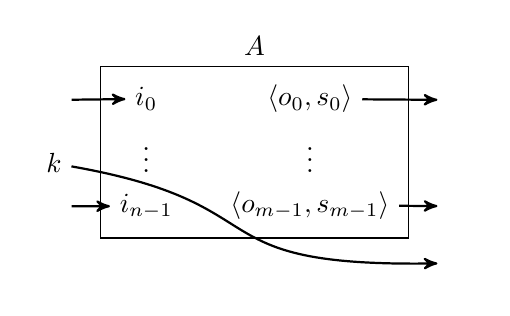
\begin{tikzpicture}

  \matrix [matrix of math nodes,column sep=0.5cm] {
    |(Ato_i_0)| \phantom{x} & |(Ai_0)| i_0 & |(Ao_0)| \langle o_0, s_0 \rangle & |(Afrom_o_0)| \phantom{x} \\
    |(A_k)| k & \vdots & \vdots & \\
    |(Ato_i_n-1)| \phantom{x} & |(Ai_n-1)| i_{n-1} & |(Ao_m-1)| \langle o_{m-1}, s_{m-1} \rangle & |(Afrom_o_m-1)| \phantom{x} \\[0.25cm]
    &&& |(A_skip)| \phantom{x} \\
  };

  \node [draw,rectangle,fit=(Ai_0) (Ai_n-1) (Ao_0) (Ao_m-1),label={[name=Alab]above:$A$}] (A) {};

  \path [draw,thick,->,>=stealth',overlay]
    (Ato_i_0)   edge (Ai_0)
    (Ato_i_n-1) edge (Ai_n-1)
    (Ao_0)      edge (Afrom_o_0)
    (Ao_m-1)    edge (Afrom_o_m-1);

  \path [draw,thick,->,>=stealth',overlay]
    (A_k) .. controls +(-10:3cm) and +($(A_skip) + (170:6cm)$) ..  (A_skip);

\end{tikzpicture}
\caption{An arbitrary fragment\label{fig:arbitrary}}
\end{figure}

\section{Atoms}

Figure~\ref{fig:atom} shows an atomic fragment, i.e., a fragment consisting of a single vertex~$v$. (Such a fragment may be produced by a literal, a character class, or the dot.) The in and out lists consist of~$v$ only, and the new edge insertion point for~$v$ is~$0$, the head of~$v$'s out edge list, because~$v$'s out edge list is empty.

\begin{figure}
\centering
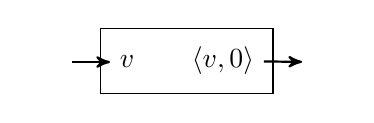
\begin{tikzpicture}

  \matrix [matrix of math nodes,column sep=0.5cm] {
    |(Ato_i_1)| \phantom{x} & |(Ai_1)| v & |(Ao_1)| \langle v, 0 \rangle & |(Afrom_o_1)| \phantom{x} \\
  };

  \node [draw,rectangle,fit=(Ai_1) (Ao_1)] (A) {};

  \path [draw,thick,->,>=stealth',overlay]
    (Ato_i_1) edge (Ai_1)
    (Ao_1)    edge (Afrom_o_1);

\end{tikzpicture}
\caption{An atom\label{fig:atom}}
\end{figure}

\section{Repetition}

Figure~\ref{fig:srep} shows how $A$ is converted to $A?$ or $A??$. In the greedy case, $A?.k = \min(A.k,A.n)$ (where $\emptyset$ is treated like $+\infty$), while in the nongreedy case $A??.k = 0$. In both cases $A?.\In = A??.\In = A.\In$, $A?.\Out = A??.\Out = A.\Out$.

\begin{figure}[h]
\centering
\subfigure[Greedy]{%
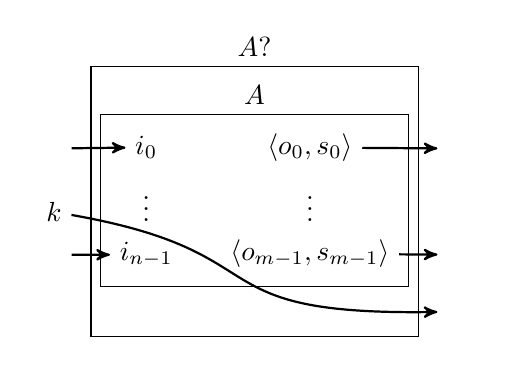
\begin{tikzpicture}

  \matrix [matrix of math nodes,column sep=0.5cm,ampersand replacement=\&] {
    |(Ato_i_0)| \phantom{x} \& |(Ai_0)| i_0 \& |(Ao_0)| \langle o_0, s_0 \rangle \& |(Afrom_o_0)| \phantom{x} \\
    |(A_k)| k \& \vdots \& \vdots \& \\
    |(Ato_i_n-1)| \phantom{x} \& |(Ai_n-1)| i_{n-1} \& |(Ao_m-1)| \langle o_{m-1}, s_{m-1} \rangle \& |(Afrom_o_m-1)| \phantom{x} \\[0.25cm]
    \& |(Abot)| \&\& |(A_skip)| \phantom{x} \\
  };

  \node [draw,rectangle,fit=(Ai_0) (Ai_n-1) (Ao_0) (Ao_m-1),label={[name=Alab]above:$A$}] (A) {};

  \path [draw,thick,->,>=stealth',overlay]
    (Ato_i_0)   edge (Ai_0)
    (Ato_i_n-1) edge (Ai_n-1)
    (Ao_0)      edge (Afrom_o_0)
    (Ao_m-1)    edge (Afrom_o_m-1);

  \path [draw,thick,->,>=stealth',overlay]
    (A_k) .. controls +(-10:3cm) and +($(A_skip) + (170:6cm)$) ..  (A_skip);

  \node [draw,rectangle,fit=(A) (Alab) (Abot),label={[name=Alab]above:$A?$}] {};

\end{tikzpicture}%
}
\subfigure[Nongreedy]{%
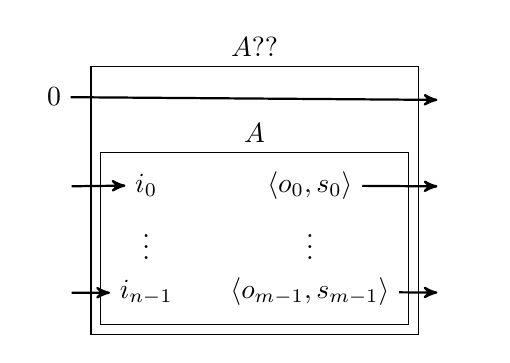
\begin{tikzpicture}

  \matrix [matrix of math nodes,column sep=0.5cm,ampersand replacement=\&] {
    \& |(Atop)| \&\& \\[-0.2cm]
    |(A_k)| 0 \&\&\& |(A_skip)| \phantom{x} \\[0.6cm]
    |(Ato_i_0)| \phantom{x} \& |(Ai_0)| i_0 \& |(Ao_0)| \langle o_0, s_0 \rangle \& |(Afrom_o_0)| \phantom{x} \\
    \& \vdots \& \vdots \& \\
    |(Ato_i_n-1)| \phantom{x} \& |(Ai_n-1)| i_{n-1} \& |(Ao_m-1)| \langle o_{m-1}, s_{m-1} \rangle \& |(Afrom_o_m-1)| \phantom{x} \\
  };

  \node [draw,rectangle,fit=(Ai_0) (Ai_n-1) (Ao_0) (Ao_m-1),label={[name=Alab]above:$A$}] (A) {};

  \path [draw,thick,->,>=stealth',overlay]
    (A_k)       edge (A_skip)
    (Ato_i_0)   edge (Ai_0)
    (Ato_i_n-1) edge (Ai_n-1)
    (Ao_0)      edge (Afrom_o_0)
    (Ao_m-1)    edge (Afrom_o_m-1);

  \node [draw,rectangle,fit=(A) (Alab) (Atop),label={[name=Alab]above:$A??$}] {};

\end{tikzpicture}%
}
\caption{Single repetition\label{fig:srep}}
\end{figure}

Figure~\ref{fig:plus} shows how $A$ is converted to $A+$ or $A+?$. Out edges are added from each $o_i$ to each $i_j$ to create the necessary loops. Adding a plus does not affect the skippability of $A$, due to the fact that matching the empty string once is the same as matching the empty string any greater number of times; hence $A?.k = A??.k = A.k$.

\begin{figure}[h]
\centering
\subfigure[Greedy]{%
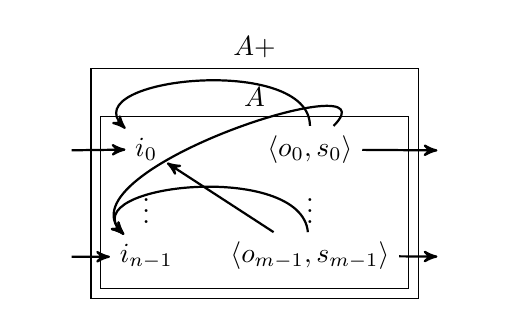
\begin{tikzpicture}

  \matrix [matrix of math nodes,column sep=0.5cm,ampersand replacement=\&] {
    |(Ato_i_0)| \phantom{x} \& |(Ai_0)| i_0 \& |(Ao_0)| \langle o_0, s_0 \rangle \& |(Afrom_o_0)| \phantom{x} \\
    \& \vdots \& \vdots \& \\
    |(Ato_i_n-1)| \phantom{x} \& |(Ai_n-1)| i_{n-1} \& |(Ao_m-1)| \langle o_{m-1}, s_{m-1} \rangle \& |(Afrom_o_m-1)| \phantom{x} \\
  };

  \node [draw,rectangle,fit=(Ai_0) (Ai_n-1) (Ao_0) (Ao_m-1),label={[name=Alab]above:$A$}] (A) {};

  \path [draw,thick,->,>=stealth',overlay]
    (Ato_i_0)   edge (Ai_0)
    (Ato_i_n-1) edge (Ai_n-1)
    (Ao_0)      edge [out=90] (Ai_0)
    (Ao_0)      edge [out=45] (Ai_n-1)
    (Ao_m-1)    edge (Ai_0)
    (Ao_m-1)    edge [out=95] (Ai_n-1)
    (Ao_0)      edge (Afrom_o_0)
    (Ao_m-1)    edge (Afrom_o_m-1);

  \node [draw,rectangle,fit=(A) (Alab),label={[name=Alab]above:$A+$}] {};

\end{tikzpicture}%
}
\subfigure[Nongreedy]{%
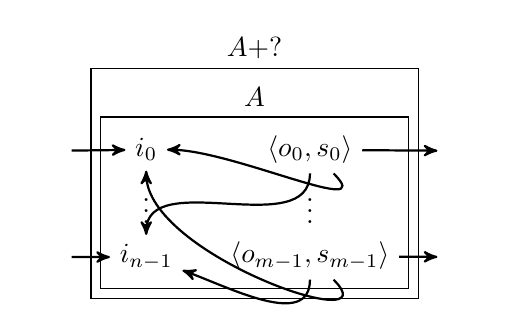
\begin{tikzpicture}

  \matrix [matrix of math nodes,column sep=0.5cm,ampersand replacement=\&] {
    |(Ato_i_0)| \phantom{x} \& |(Ai_0)| i_0 \& |(Ao_0)| \langle o_0, s_0 \rangle \& |(Afrom_o_0)| \phantom{x} \\
    \& \vdots \& \vdots \& \\
    |(Ato_i_n-1)| \phantom{x} \& |(Ai_n-1)| i_{n-1} \& |(Ao_m-1)| \langle o_{m-1}, s_{m-1} \rangle \& |(Afrom_o_m-1)| \phantom{x} \\
  };

  \node [draw,rectangle,fit=(Ai_0) (Ai_n-1) (Ao_0) (Ao_m-1),label={[name=Alab]above:$A$}] (A) {};

  \path [draw,thick,->,>=stealth',overlay]
    (Ato_i_0)   edge (Ai_0)
    (Ato_i_n-1) edge (Ai_n-1)
    (Ao_0)      edge [out=-45,in=0] (Ai_0)
    (Ao_0)      edge [out=-90,in=90] (Ai_n-1)
    (Ao_m-1)    edge [out=-45,in=-90] (Ai_0)
    (Ao_m-1)    edge [out=-90,in=-20] (Ai_n-1)

    (Ao_0)      edge (Afrom_o_0)
    (Ao_m-1)    edge (Afrom_o_m-1);

  \node [draw,rectangle,fit=(A) (Alab),label={[name=Alab]above:$A+?$}] {};

\end{tikzpicture}%
}
\caption{Unbounded repetition\label{fig:plus}}
\end{figure}

No diagrams are given for the conversion of $A$ to $A*$ or $A*?$, as these are equivalent to $(A+)?$ and $(A+?)??$, respectively, so can be constructed from the above. 

\section{Alternation}

Figure~\ref{fig:alt} shows how $A|B$ is formed from $A$ and $B$. In all cases, $A|B.\In = A.\In + B.\In$, $A|B.\Out = A.\Out + B.\Out$. Finally,
\[ A|B.k = \begin{cases}
  \emptyset & \text{if } A.k = B.k = \emptyset,\\
  A.k       & \text{if } A.k \ne \emptyset,\\
  \lvert A.\In\rvert + B.k & \text{if } B.k \ne \emptyset.
\end{cases}\]
The intuition behind the skippability for $A|B$ is as follows: If a fragment is skippable, that means it matches the empty string. If $A$ matches the empty string, since $A$ matches for $A$ have priority over matches for $B$, the empty string should be matched by $A|B$ with the priority $A$ gives it. Otherwise, if $A$ is not skippable, but $B$ is, since $A|B.\In$ is just $B.\In$ with $A.\In$ prepended to it, and $B.k$ is an insertion position, $B.k$ needs to be shifted by the size of $A.\In$ to give us $A|B.k$.

\begin{figure}
\centering
\subfigure[$A.k = B.k = \emptyset$]{%
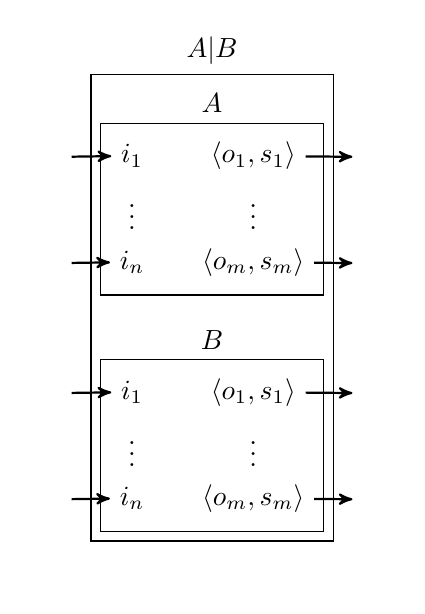
\begin{tikzpicture}[baseline=(current bounding box.north)]

  \matrix [matrix of math nodes,column sep=0.5cm,ampersand replacement=\&] at (0,1.5) {
    |(Ato_i_1)| \phantom{x} \& |(Ai_1)| i_1 \& |(Ao_1)| \langle o_1, s_1 \rangle \& |(Afrom_o_1)| \phantom{x} \\
    \& \vdots \& \vdots \& \\
    |(Ato_i_n)| \phantom{x} \& |(Ai_n)| i_n \& |(Ao_m)| \langle o_m, s_m \rangle \& |(Afrom_o_m)| \phantom{x} \\
  };

  \node [draw,rectangle,fit=(Ai_1) (Ai_n) (Ao_1) (Ao_m),label={[name=Alab]above:$A$}] (A) {};

  \path [draw,thick,->,>=stealth',overlay]
    (Ato_i_1) edge (Ai_1)
    (Ato_i_n) edge (Ai_n)
    (Ao_1)    edge (Afrom_o_1)
    (Ao_m)    edge (Afrom_o_m);

  \matrix [matrix of math nodes,column sep=0.5cm,ampersand replacement=\&] at (0,-1.5) {
    |(Bto_i_1)| \phantom{x} \& |(Bi_1)| i_1 \& |(Bo_1)| \langle o_1, s_1 \rangle \& |(Bfrom_o_1)| \phantom{x} \\
    \& \vdots \& \vdots \& \\
    |(Bto_i_n)| \phantom{x} \& |(Bi_n)| i_n \& |(Bo_m)| \langle o_m, s_m \rangle \& |(Bfrom_o_m)| \phantom{x} \\
  };

  \node [draw,rectangle,fit=(Bi_1) (Bi_n) (Bo_1) (Bo_m),label={[name=Blab]above:$B$}] (B) {};

   \path [draw,thick,->,>=stealth',overlay]
    (Bto_i_1) edge (Bi_1)
    (Bto_i_n) edge (Bi_n)
    (Bo_1)    edge (Bfrom_o_1)
    (Bo_m)    edge (Bfrom_o_m);

  \node [draw,rectangle,fit=(A) (Alab) (B) (Blab),label=above:$A|B$] (AB) {};

  \node [below=0.75\baselineskip of AB] {};
\end{tikzpicture}
}
\subfigure[$A.k \ne \emptyset$]{%
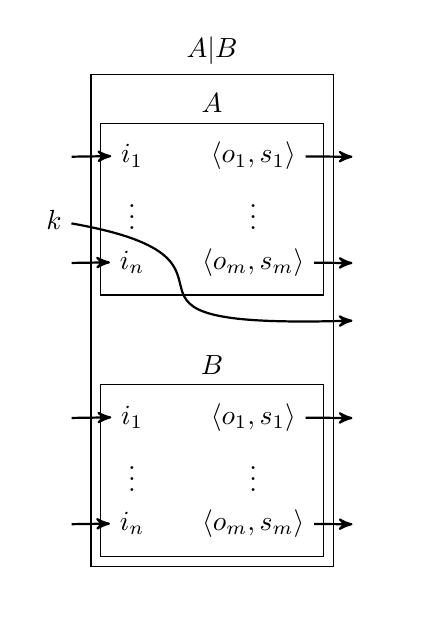
\begin{tikzpicture}[baseline=(current bounding box.north)]

  \matrix [matrix of math nodes,column sep=0.5cm,ampersand replacement=\&] at (0,1.5) {
    |(Ato_i_1)| \phantom{x} \& |(Ai_1)| i_1 \& |(Ao_1)| \langle o_1, s_1 \rangle \& |(Afrom_o_1)| \phantom{x} \\
    |(A_k)| k \& \vdots \& \vdots \& \\
    |(Ato_i_n)| \phantom{x} \& |(Ai_n)| i_n \& |(Ao_m)| \langle o_m, s_m \rangle \& |(Afrom_o_m)| \phantom{x} \\[0.25cm]
    \&\&\& |(A_skip)| \phantom{x} \\
  };

  \node [draw,rectangle,fit=(Ai_1) (Ai_n) (Ao_1) (Ao_m),label={[name=Alab]above:$A$}] (A) {};

  \path [draw,thick,->,>=stealth',overlay]
    (Ato_i_1) edge (Ai_1)
    (Ato_i_n) edge (Ai_n)
    (Ao_1)    edge (Afrom_o_1)
    (Ao_m)    edge (Afrom_o_m);

  \path [draw,thick,->,>=stealth',overlay]
    (A_k) .. controls +(-10:3cm) and +($(A_skip) + (185:6cm)$) ..  (A_skip);

  \matrix [matrix of math nodes,column sep=0.5cm,ampersand replacement=\&] at (0,-1.5) {
    |(Bto_i_1)| \phantom{x} \& |(Bi_1)| i_1 \& |(Bo_1)| \langle o_1, s_1 \rangle \& |(Bfrom_o_1)| \phantom{x} \\
    \& \vdots \& \vdots \& \\
    |(Bto_i_n)| \phantom{x} \& |(Bi_n)| i_n \& |(Bo_m)| \langle o_m, s_m \rangle \& |(Bfrom_o_m)| \phantom{x} \\
  };

  \node [draw,rectangle,fit=(Bi_1) (Bi_n) (Bo_1) (Bo_m),label={[name=Blab]above:$B$}] (B) {};

   \path [draw,thick,->,>=stealth',overlay]
    (Bto_i_1) edge (Bi_1)
    (Bto_i_n) edge (Bi_n)
    (Bo_1)    edge (Bfrom_o_1)
    (Bo_m)    edge (Bfrom_o_m);

  \node [draw,rectangle,fit=(A) (Alab) (B) (Blab),label=above:$A|B$] (AB) {};

  \node [below=0.25\baselineskip of AB] {};
\end{tikzpicture}
}
\subfigure[$A.k = \emptyset, B.k \ne \emptyset$]{%
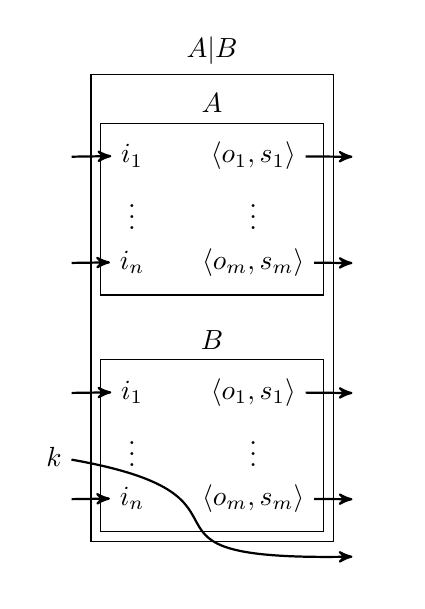
\begin{tikzpicture}

  \matrix [matrix of math nodes,column sep=0.5cm,ampersand replacement=\&] at (0,1.5) {
    |(Ato_i_1)| \phantom{x} \& |(Ai_1)| i_1 \& |(Ao_1)| \langle o_1, s_1 \rangle \& |(Afrom_o_1)| \phantom{x} \\
    \& \vdots \& \vdots \& \\
    |(Ato_i_n)| \phantom{x} \& |(Ai_n)| i_n \& |(Ao_m)| \langle o_m, s_m \rangle \& |(Afrom_o_m)| \phantom{x} \\[0.25cm]
    \&\&\& |(A_skip)| \phantom{x} \\
  };

  \node [draw,rectangle,fit=(Ai_1) (Ai_n) (Ao_1) (Ao_m),label={[name=Alab]above:$A$}] (A) {};

  \path [draw,thick,->,>=stealth',overlay]
    (Ato_i_1) edge (Ai_1)
    (Ato_i_n) edge (Ai_n)
    (Ao_1)    edge (Afrom_o_1)
    (Ao_m)    edge (Afrom_o_m);

  \matrix [matrix of math nodes,column sep=0.5cm,ampersand replacement=\&] at (0,-1.5) {
    |(Bto_i_1)| \phantom{x} \& |(Bi_1)| i_1 \& |(Bo_1)| \langle o_1, s_1 \rangle \& |(Bfrom_o_1)| \phantom{x} \\
    |(B_k)| k \& \vdots \& \vdots \& \\
    |(Bto_i_n)| \phantom{x} \& |(Bi_n)| i_n \& |(Bo_m)| \langle o_m, s_m \rangle \& |(Bfrom_o_m)| \phantom{x} \\[0.25cm]
    \&\&\& |(B_skip)| \phantom{x} \\
  };

  \node [draw,rectangle,fit=(Bi_1) (Bi_n) (Bo_1) (Bo_m),label={[name=Blab]above:$B$}] (B) {};

   \path [draw,thick,->,>=stealth',overlay]
    (Bto_i_1) edge (Bi_1)
    (Bto_i_n) edge (Bi_n)
    (Bo_1)    edge (Bfrom_o_1)
    (Bo_m)    edge (Bfrom_o_m);

  \path [draw,thick,->,>=stealth',overlay]
    (B_k) .. controls +(-10:3cm) and +($(B_skip) + (155:6cm)$) .. (B_skip);

  \node [draw,rectangle,fit=(A) (Alab) (B) (Blab),label=above:$A|B$] (AB) {};

\end{tikzpicture}
}
\caption{Alternation\label{fig:alt}}
\end{figure}

\pagebreak
\section{Concatenation}

Figure~\ref{fig:concat} shows how $AB$ is formed from $A$ and $B$. There are four cases, depending on whether either $A$ or $B$ is skippable. In what follows, the bracket notation indicates array slices.
\begin{align*}
  AB.k &= \begin{cases}
    A.k + B.k & \text{if } A.k \ne \emptyset \text{ and } B.k \ne \emptyset,\\
    \emptyset & \text{otherwise.}
  \end{cases}
  \\
  AB.\In &= \begin{cases}
    A.\In[0:A.k-1] + B.\In + A.\In[A.k:\lvert A.\In\rvert] & \text{if } A.k \ne \emptyset,\\
    A.\In & \text{otherwise.}\\
  \end{cases}
  \\
  AB.\Out &= \begin{cases}
    B.\Out + \{\langle v,s\rangle \mid \langle v,s'\rangle \in A.\Out \wedge s = \lvert v.\Out \rvert + B.k \} & \text{if } B.k \ne \emptyset,\\
    B.\Out & \text{otherwise.}
  \end{cases}
\end{align*}
The skippability of $A$ determines $AB.\In$; the skippability of $B$ determines $AB.\Out$; the skippability of $A$ and $B$ jointly determine the skippability of $AB.k$.


\begin{figure}
\centering
\subfigure[$A.k = B.k = \emptyset$]{%
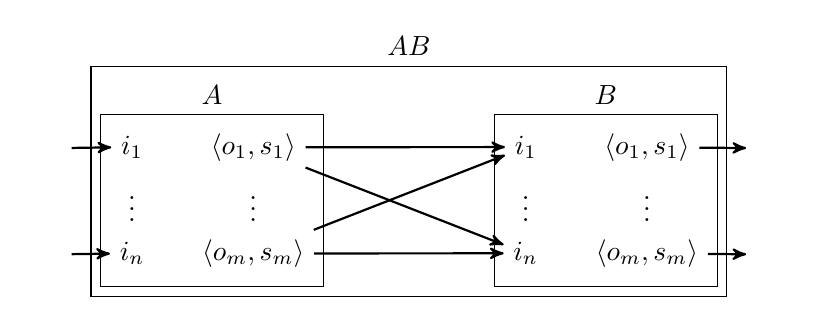
\begin{tikzpicture}

  \matrix [matrix of math nodes,column sep=0.5cm,ampersand replacement=\&] at (-2.5,0) {
    |(Ato_i_1)| \phantom{x} \& |(Ai_1)| i_1 \& |(Ao_1)| \langle o_1, s_1 \rangle \& |(Afrom_o_1)| \phantom{x} \\
    \& \vdots \& \vdots \& \\
    |(Ato_i_n)| \phantom{x} \& |(Ai_n)| i_n \& |(Ao_m)| \langle o_m, s_m \rangle \& |(Afrom_o_m)| \phantom{x} \\
  };

  \node [draw,rectangle,fit=(Ai_1) (Ai_n) (Ao_1) (Ao_m),label={[name=Alab]above:$A$}] (A) {};

  \path [draw,thick,->,>=stealth',overlay]
    (Ato_i_1) edge (Ai_1)
    (Ato_i_n) edge (Ai_n);

  \matrix [matrix of math nodes,column sep=0.5cm,ampersand replacement=\&] at (2.5,0) {
    |(Bto_i_1)| \phantom{x} \& |(Bi_1)| i_1 \& |(Bo_1)| \langle o_1, s_1 \rangle \& |(Bfrom_o_1)| \phantom{x} \\
    \& \vdots \& \vdots \& \\
    |(Bto_i_n)| \phantom{x} \& |(Bi_n)| i_n \& |(Bo_m)| \langle o_m, s_m \rangle \& |(Bfrom_o_m)| \phantom{x} \\
  };

  \node [draw,rectangle,fit=(Bi_1) (Bi_n) (Bo_1) (Bo_m),label={[name=Blab]above:$B$}] (B) {};

  \path [draw,thick,->,>=stealth',overlay]
    (Bo_1) edge (Bfrom_o_1)
    (Bo_m) edge (Bfrom_o_m);

  \path [draw,thick,->,>=stealth']
    (Ao_1) edge (Bi_1)
    (Ao_1) edge (Bi_n)
    (Ao_m) edge (Bi_1)
    (Ao_m) edge (Bi_n);

  \node [draw,rectangle,fit=(A) (Alab) (B) (Blab),label=above:$AB$] (AB) {};

\end{tikzpicture}
}
\subfigure[$A.k = \emptyset, B.k \ne \emptyset$]{%
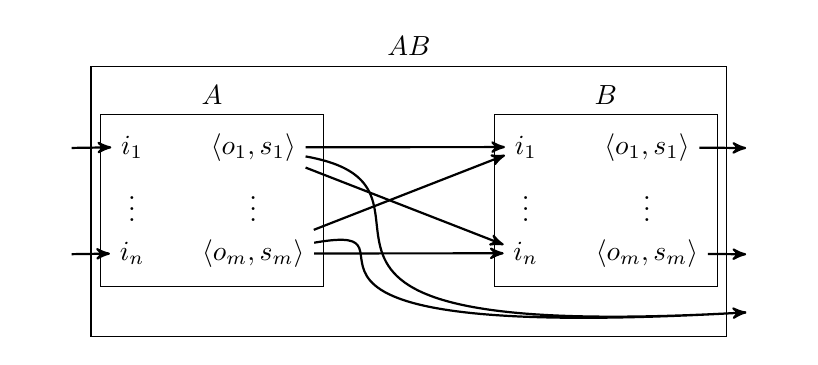
\begin{tikzpicture}

  \matrix [matrix of math nodes,column sep=0.5cm,anchor=north,ampersand replacement=\&] at (-2.5,0) {
    |(Ato_i_1)| \phantom{x} \& |(Ai_1)| i_1 \& |(Ao_1)| \langle o_1, s_1 \rangle \& |(Afrom_o_1)| \phantom{x} \\
    \& \vdots \& \vdots \& \\
    |(Ato_i_n)| \phantom{x} \& |(Ai_n)| i_n \& |(Ao_m)| \langle o_m, s_m \rangle \& |(Afrom_o_m)| \phantom{x} \\
  };

  \node [draw,rectangle,fit=(Ai_1) (Ai_n) (Ao_1) (Ao_m),label={[name=Alab]above:$A$}] (A) {};

  \path [draw,thick,->,>=stealth',overlay]
    (Ato_i_1) edge (Ai_1)
    (Ato_i_n) edge (Ai_n);

  \matrix [matrix of math nodes,column sep=0.5cm,anchor=north,ampersand replacement=\&] at (2.5,0) {
    |(Bto_i_1)| \phantom{x} \& |(Bi_1)| i_1 \& |(Bo_1)| \langle o_1, s_1 \rangle \& |(Bfrom_o_1)| \phantom{x} \\
    \& \vdots \& \vdots \& \\
    |(Bto_i_n)| \phantom{x} \& |(Bi_n)| i_n \& |(Bo_m)| \langle o_m, s_m \rangle \& |(Bfrom_o_m)| \phantom{x} \\[0.25cm]
    \&\& |(B_skip)| \& |(Bfrom_skip)| \phantom{x} \\
  };

  \node [draw,rectangle,fit=(Bi_1) (Bi_n) (Bo_1) (Bo_m),label={[name=Blab]above:$B$}] (B) {};

  \path [draw,thick,->,>=stealth',overlay]
    (Bo_1) edge (Bfrom_o_1)
    (Bo_m) edge (Bfrom_o_m);

  \path [draw,thick,->,>=stealth']
    (Ao_1) edge (Bi_1)
    (Ao_1) edge (Bi_n)
    (Ao_m) edge (Bi_1)
    (Ao_m) edge (Bi_n);

  \path [draw,thick,->,>=stealth',overlay]
    (Ao_1) .. controls +(-10:3cm) and +($(Bfrom_skip) + (170:12cm)$) .. (Bfrom_skip)
    (Ao_m) .. controls +(10:2.5cm) and +($(Bfrom_skip) + (170:12cm)$) .. (Bfrom_skip);


  \node [draw,rectangle,fit=(A) (Alab) (B) (Blab) (B_skip),label=above:$AB$] (AB) {};

\end{tikzpicture}
}
\subfigure[$A.k \ne \emptyset, B.k = \emptyset$]{%
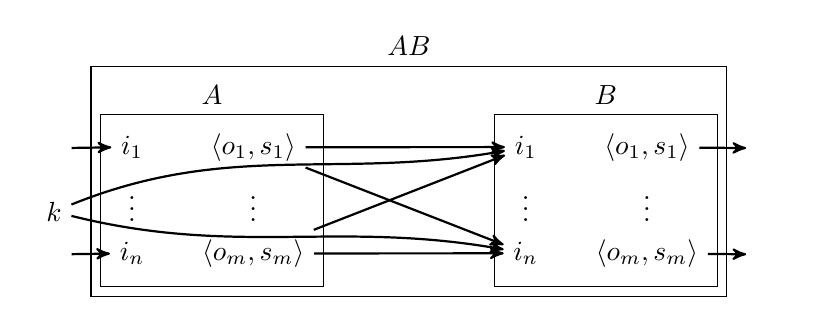
\begin{tikzpicture}
  \matrix [matrix of math nodes,column sep=0.5cm,ampersand replacement=\&] at (-2.5,0) {
    |(Ato_i_1)| \phantom{x} \& |(Ai_1)| i_1 \& |(Ao_1)| \langle o_1, s_1 \rangle \& |(Afrom_o_1)| \phantom{x} \\
    |(A_skip)| k \& \vdots \& \vdots \& \\
    |(Ato_i_n)| \phantom{x} \& |(Ai_n)| i_n \& |(Ao_m)| \langle o_m, s_m \rangle \& |(Afrom_o_m)| \phantom{x} \\
  };

  \node [draw,rectangle,fit=(Ai_1) (Ai_n) (Ao_1) (Ao_m),label={[name=Alab]above:$A$}] (A) {};

  \path [draw,thick,->,>=stealth',overlay]
    (Ato_i_1) edge (Ai_1)
    (Ato_i_n) edge (Ai_n);

  \matrix [matrix of math nodes,column sep=0.5cm,ampersand replacement=\&] at (2.5,0) {
    |(Bto_i_1)| \phantom{x} \& |(Bi_1)| i_1 \& |(Bo_1)| \langle o_1, s_1 \rangle \& |(Bfrom_o_1)| \phantom{x} \\
    \& \vdots \& \vdots \& \\
    |(Bto_i_n)| \phantom{x} \& |(Bi_n)| i_n \& |(Bo_m)| \langle o_m, s_m \rangle \& |(Bfrom_o_m)| \phantom{x} \\
  };

  \node [draw,rectangle,fit=(Bi_1) (Bi_n) (Bo_1) (Bo_m),label={[name=Blab]above:$B$}] (B) {};

  \path [draw,thick,->,>=stealth',overlay]
    (Bo_1) edge (Bfrom_o_1)
    (Bo_m) edge (Bfrom_o_m);

  \path [draw,thick,->,>=stealth']
    (Ao_1) edge (Bi_1)
    (Ao_1) edge (Bi_n)
    (Ao_m) edge (Bi_1)
    (Ao_m) edge (Bi_n);

  \node [draw,rectangle,fit=(A) (Alab) (B) (Blab),label=above:$AB$] (AB) {};

  \path [draw,thick,->,>=stealth',overlay]
    (A_skip) edge [out=22,in=190] (Bi_1)
    (A_skip) edge [out=-14,in=170] (Bi_n);

\end{tikzpicture}
}
\subfigure[$A.k \ne \emptyset, B.k \ne \emptyset$]{%
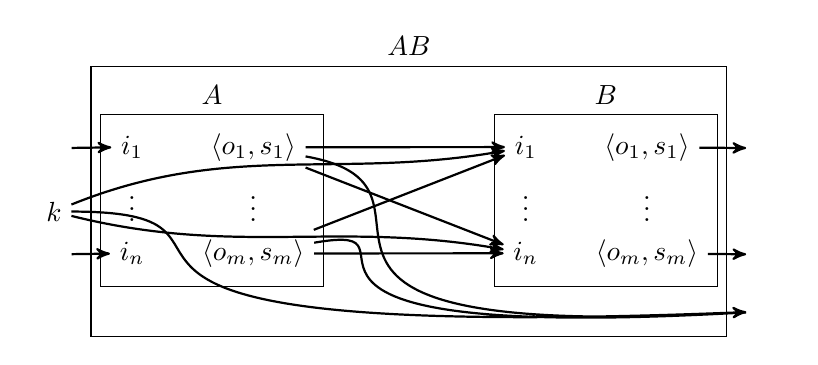
\begin{tikzpicture}
  \matrix [matrix of math nodes,column sep=0.5cm,anchor=north,ampersand replacement=\&] at (-2.5,0) {
    |(Ato_i_1)| \phantom{x} \& |(Ai_1)| i_1 \& |(Ao_1)| \langle o_1, s_1 \rangle \& |(Afrom_o_1)| \phantom{x} \\
    |(A_skip)| k \& \vdots \& \vdots \& \\
    |(Ato_i_n)| \phantom{x} \& |(Ai_n)| i_n \& |(Ao_m)| \langle o_m, s_m \rangle \& |(Afrom_o_m)| \phantom{x} \\
  };

  \node [draw,rectangle,fit=(Ai_1) (Ai_n) (Ao_1) (Ao_m),label={[name=Alab]above:$A$}] (A) {};

  \path [draw,thick,->,>=stealth',overlay]
    (Ato_i_1) edge (Ai_1)
    (Ato_i_n) edge (Ai_n);

  \matrix [matrix of math nodes,column sep=0.5cm,anchor=north,ampersand replacement=\&] at (2.5,0) {
    |(Bto_i_1)| \phantom{x} \& |(Bi_1)| i_1 \& |(Bo_1)| \langle o_1, s_1 \rangle \& |(Bfrom_o_1)| \phantom{x} \\
    \& \vdots \& \vdots \& \\
    |(Bto_i_n)| \phantom{x} \& |(Bi_n)| i_n \& |(Bo_m)| \langle o_m, s_m \rangle \& |(Bfrom_o_m)| \phantom{x} \\[0.25cm]
    \&\& |(B_skip)| \& |(Bfrom_skip)| \phantom{x} \\
  };

  \node [draw,rectangle,fit=(Bi_1) (Bi_n) (Bo_1) (Bo_m),label={[name=Blab]above:$B$}] (B) {};

  \path [draw,thick,->,>=stealth',overlay]
    (Bo_1) edge (Bfrom_o_1)
    (Bo_m) edge (Bfrom_o_m);

  \path [draw,thick,->,>=stealth']
    (Ao_1) edge (Bi_1)
    (Ao_1) edge (Bi_n)
    (Ao_m) edge (Bi_1)
    (Ao_m) edge (Bi_n);

  \node [draw,rectangle,fit=(A) (Alab) (B) (Blab) (B_skip),label=above:$AB$] (AB) {};

  \path [draw,thick,->,>=stealth',overlay]
    (A_skip) edge [out=22,in=190] (Bi_1)
    (A_skip) edge [out=-14,in=170] (Bi_n);

  \path [draw,thick,->,>=stealth',overlay]
    (Ao_1) .. controls +(-10:3cm) and +($(Bfrom_skip) + (170:12cm)$) .. (Bfrom_skip)
    (Ao_m) .. controls +(10:2.5cm) and +($(Bfrom_skip) + (170:12cm)$) .. (Bfrom_skip)
    (A_skip) .. controls +(0:3.25cm) and +($(Bfrom_skip) + (172:15cm)$) .. (Bfrom_skip);

\end{tikzpicture}
}
\caption{Concatenation\label{fig:concat}}
\end{figure}

\end{document}
